\documentclass[10pt,a4paper]{article}
\usepackage[utf8]{inputenc}
\usepackage[english]{babel}
\usepackage{amsmath}
\usepackage{amsfonts}
\usepackage{amssymb}
\usepackage{graphicx}
\usepackage{geometry}
\usepackage{footnote}
\usepackage{pdfpages}
\usepackage[toc,page]{appendix}
\usepackage{placeins}

\makesavenoteenv{tabular}

\title{PostCardBuddy}
\author{Team C}

\begin{document}
\begin{titlepage}
\newgeometry{left=2cm,top=1cm,right=2cm}
\newcommand{\HRule}{\rule{\linewidth}{0.5mm}}


\begin{flushright}
November 15, 2015 v2.0\\[3cm]
\end{flushright}


\centering
\textsc{\LARGE Team C}\\[0.5cm]

\HRule \\[0.4cm]
{ \huge \bfseries PostCardBuddy}\\[0.3cm]
{\Large \bfseries Project Mission}\\[0.4cm] % Title of your document
\HRule \\[1.5cm]

\vfill
\begin{flushleft}
%Authors, write on separate lines
\textit{Authors of this document:}\\
Emma Albertz\\
Caroline Brandberg\\
Linnéa Claesson\\
Billy Johansson\\
Johan Ju\\
Jacob Mejvik\\
Carl Rynegardh
\end{flushleft}

\end{titlepage}
\pagenumbering{gobble}



%\begin{center}
%\textit{\large Version History}
%
%    \begin{tabular}{ | l | l | l | p{5cm} |}
%    \hline
%    \textbf{Version} & \textbf{Date} & \textbf{Responsible} & \textbf{Description} \\ \hline
%    1.0 & 2015-10-14 & EA, LC & Baseline\\ \hline
%    \end{tabular}
%\end{center}



\setcounter{tocdepth}{2}
\tableofcontents
\newpage
\pagenumbering{arabic}




%--------------------------------------------------------------------------%
%--------------------- Background------------------------------------------%
%--------------------------------------------------------------------------%
\section{Background}
% Background and other information from PMv1
% What is the project about?

In today's society there are constantly more and more things to consider, which causes a lot of stress for many people. Even when you are on vacation to recover, there are issues you can encounter which cause stress. With PostCardBuddy we aim to reduce your stress level when on vacation by introducing a simple and convenient way to let the people back home know you are thinking of them. 


\section{Main Goals and System Context}
% Vad ska appen kunna göra/funktionalitet och vart/hur ska den användas?
The goal of this project is to develop a mobile application, which lets the user create postcards. The postcards can then be sent to anyone, both digitally by email or as a physical copy, from the application. 

This application aims to reduce stress for people on vacation and its functionality should also include the following:

\begin{itemize}
\item Create postcard consisting of a front and back
\begin{description}
\item[Front] Image, one or multiple
\item[Back] Greeting to and address of recipient
\end{description}
\item Take a picture with the camera (within the application) or use an existing one, either from the phone's gallery or application's gallery
\item Simple image editing
\item Write a greeting in the application, take a photograph of handwritten text or use auto-generated greetings
\item Image and greetings suggestions based on current GPS location
\item Possibility to save images, greetings and postcards so they can be re-used easily
\item History of sent postcards
\item Access recipients from phone's contact list or enter manually
\item Multiple recipients
\item Favourites; both contacts frequently used and marked manually by user
\item Options for choosing size and quality of physical postcard to be sent
\item Confirmation of order
\item Payment within application
\end{itemize}


\section{Participants and Stakeholders}
% What will the customer team spend their time on? Elicitation?
% Leverantör, kunden, mobilanvändare
The end user of this application will be vacationing mobile users. A chosen group will be used to evaluate prototypes of the product, to make sure it is easy to use and has the desired functionality. They might also be asked to take a survey to answer further questions.

Other stakeholders are the potential suppliers of the physical postcards, who will print out and deliver them to the recipients. Therefore, they will be used for the requirements concerning the delivery of the postcards. These requirements will include, among others, the required format of the postcards to be printed and price. Potential suppliers will be contacted for interviews.

Team A is the key customer for this project and they will be considered a supplier of the physical postcards. They will be used for the elicitation process, specifically for requirements concerning functionality and quality of the product. This will be done by interviews or using a focus group. 

There are similar existing products already on the market, a document study will therefore be conducted to elicit additional functional and quality requirements. 

Additional potential stakeholders are advertisers, travel companies and mobile manufacturers but they will not be contacted during the course of this project.

Figure~\ref{fig:stake} shows how a mobile user and a supplier will interact with the application. 

\begin{figure}[h!]
\centering
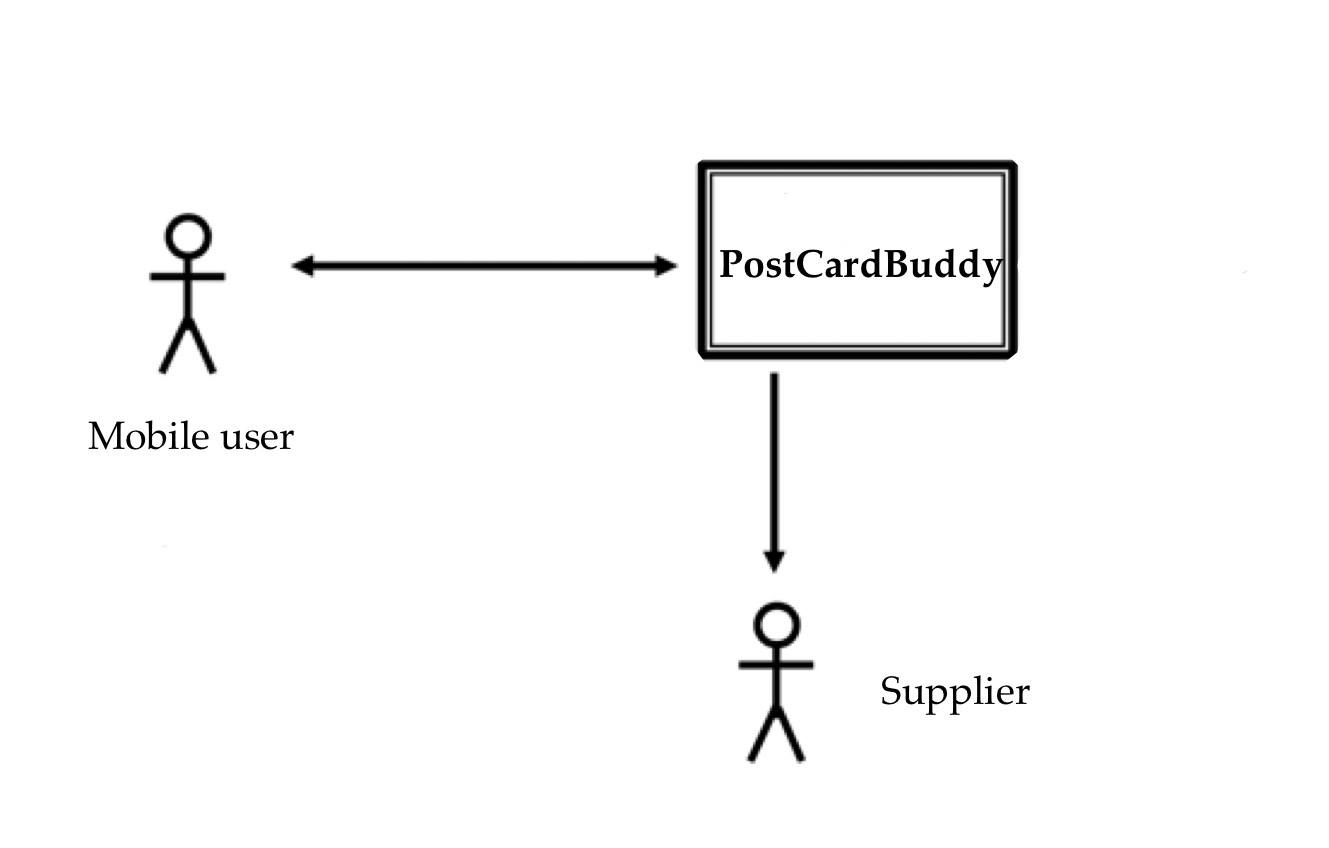
\includegraphics[width=0.7\textwidth]{im.jpg}
\caption{Interaction with the application.}
\label{fig:stake}
\end{figure}

\section{Activities and Deliverables}
% Description of planned activities and deliverables with deadlines (see Course program) 

In table~\ref{table:deliv} the deliverables and their respective deadlines are shown for each phase of the project. 

Table~\ref{table:meet} displays other activities planned during this project. The weekly group meetings will be held on Mondays at 1:15 p.m. The intention of these meetings is to give an overview of the progress of the project and what is to be done in the upcoming week. All group members have exercises scheduled on Tuesdays at 3:15 p.m., which will be an additional opportunity for the group to work on the project. 

The meetings with the supervisor will be used to report status, discuss challenges/questions and plans for the project. The group should meet up prior to each supervisor meeting to assess what needs to be brought up to make the meeting as efficient as possible. 

A presentation of the project is scheduled for the last week.



\begin{table}[h!]
\centering
\caption{Deliverables and deadlines of each phase of the project.}
\label{table:deliv}
\begin{tabular}{|l|l|l|} \hline
\textbf{Phase} & \textbf{Deliverables} & \textbf{Deadline}\\ \hline
Definition & Project Mission v1 & Week 1: Friday 09:00\\ \hline
Planning & Project Mission v2 & Week 3: Monday 09:00\\ \hline
Iteration 1 & Release R1 & Week 4: Monday 09:00\\ \hline
Iteration 2 & Release R2 & Week 6: Monday 09:00\\ \hline
& Validation Checklist & Week 6: Monday 09:00\\ \hline
& Validation Report & Week 6: Friday 09:00\\ \hline
Iteration 3 & Conference Presentation & Week 6: Sunday 15:00\\ \hline
& Release R3 & Week 7: Sunday 23:59\\ \hline
\end{tabular}\\
\end{table}

\begin{table}[h!]
\centering
\caption{Planned activities.}
\label{table:meet}
\begin{tabular}{|l|c|c|c|c|c|c|c|} \hline
&Week 1 & Week 2 & Week 3 & Week 4 & Week 5 & Week 6 & Week 7\\ \hline
Group meeting & X &X&X&X&X&X&X\\ \hline
Supervisor meeting &&X&&X&&X&\\ \hline
Exercise & X &X&X&X&X&X&X\\ \hline
Presentation &&&&&&&X\\ \hline 
\end{tabular}\\
\end{table}


\section{Time Schedule}
% Diagram showing the planned time per week and participant
See appendix for Gantt and Weekly schedule of this project.


\section{Project Team Members}
% Responsibilities of project members
The management roles of the project are the following:

\begin{description}
\item[P3RM] Project, Process, Prioritization, and Release Manager
\item[SCCVM] Stakeholder, Customer Communication and Validation Manager
\item[TDEVM] Tools, Documents, Experiences and Version Manager 
\item[EPM] Elicitation and Prototyping Manager
\item[QRM] Quality Requirements Manager
\item[DRM] Data Requirements Manager
\end{description}

The roles and contact information to each team member can be found in table~\ref{table:roles}. Each manager is responsible for planning and coordinating the tasks of his or her specific area and divide the tasks appropriately within the team.

\begin{table}[h!]
\centering
\caption{Roles of project members.}
\label{table:roles}
\begin{tabular}{|l|l|l|} \hline
P3RM & Linnéa Claesson & eko11lcl@student.lu.se\\ \hline
SCCVM & Caroline Brandberg & elt12cbr@student.lu.se\\ \hline
TDEVM & Jacob Mejvik & jur05jme@student.lu.se\\ \hline
EPM & Emma Albertz & ine11eal@student.lu.se\\ \hline
EPM & Carl Rynegardh & elt12cry@student.lu.se\\ \hline
QRM & Johan Ju & elt12jju@student.lu.se\\ \hline
DRM & Billy Johansson & ama10bjo@student.lu.se\\ \hline

\end{tabular}\\
\end{table}
\FloatBarrier

\newpage
\begin{appendices}
\section{Time Schedule}

\subsection{Gantt Schedule}
\begin{figure}[h!]
\centering
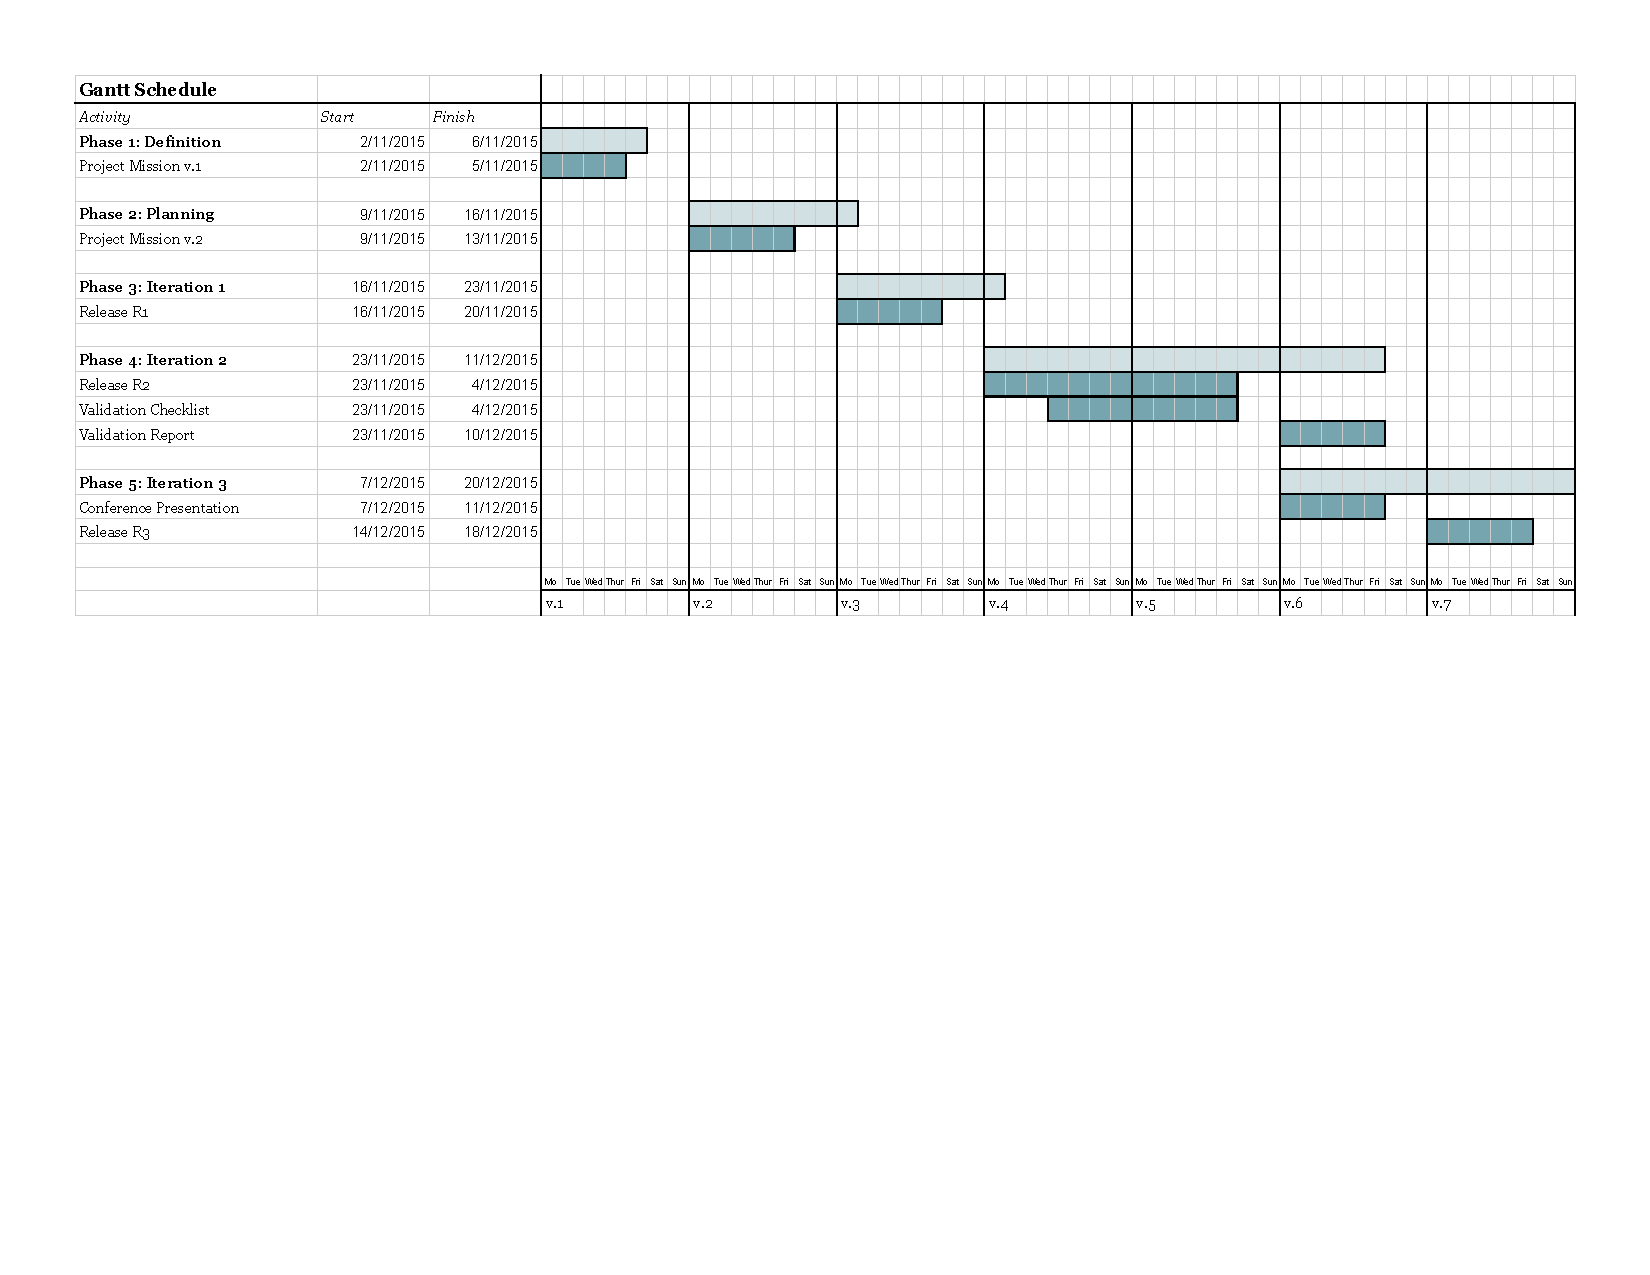
\includegraphics[width=1.1\textwidth]{Gantt.pdf}
\end{figure}
\FloatBarrier

\subsection{Weekly Schedule}
\begin{figure}[h!]
\centering
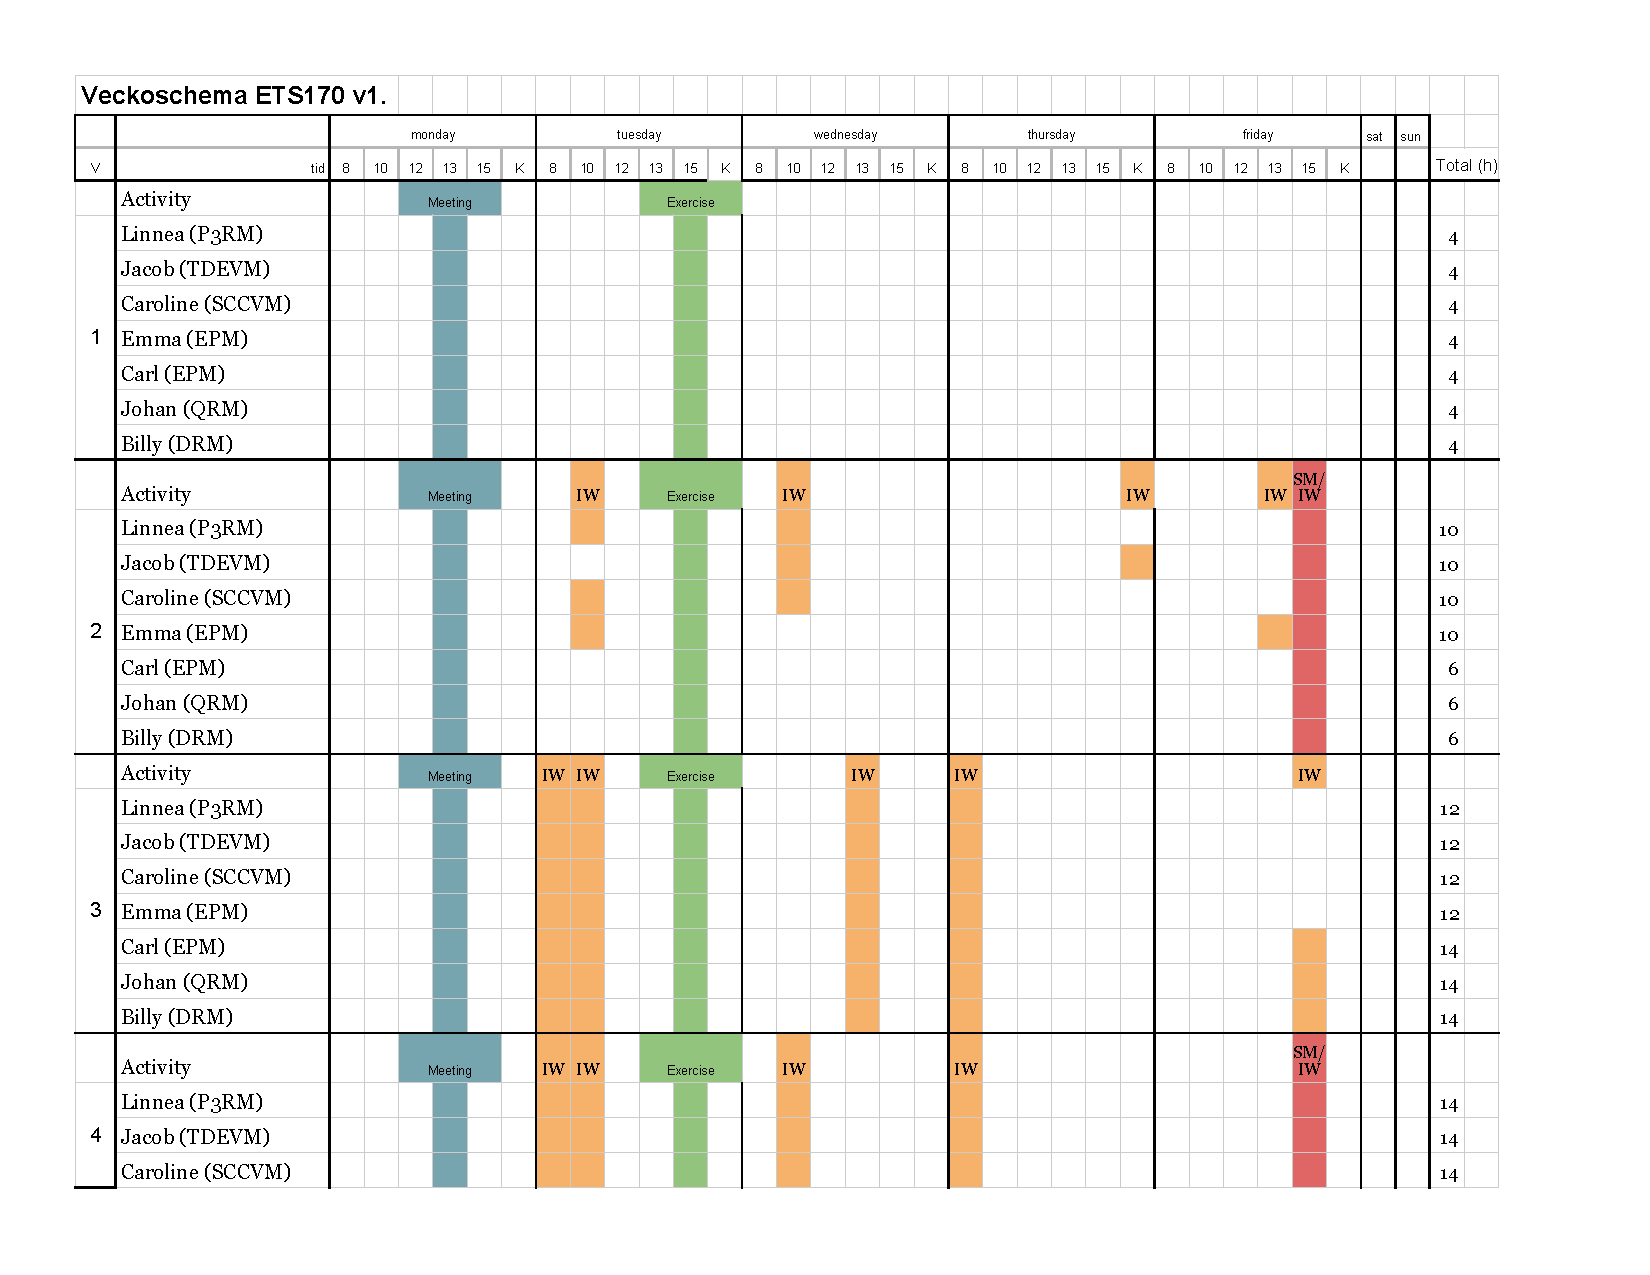
\includegraphics[width=1.1\textwidth, trim=0mm 0mm 0mm 0mm, clip]{Veckoschema.pdf}
\end{figure}

\begin{figure}[h!]
\centering
\includegraphics[page=2, width=1.1\textwidth, trim=0mm 0mm 0mm 0mm, clip]{Veckoschema.pdf}
\end{figure}

\begin{figure}[h!]
\centering
\includegraphics[page=3, width=1.1\textwidth, trim=0mm 140mm 0mm 0mm, clip]{Veckoschema.pdf}
\end{figure}


\end{appendices}
\end{document}

